\section{Analysis}\label{sect:analysis}

\lhead{\textit{Analysis}}
\subsection{Fixed Points Analysis} \label{sect:fixed_point_analysis}

It can be clearly seen that the models above represent discrete time mappings. As such, it is therefore possible to identify fixed points to better understand the behaviour of some of the models. As in~\cite{Hegselmann2002Opinion}, it is challenging to provide analytical insights for each of these models, though the Open model, introduced in~\cref{sect:speaker_models}, provides a relatively simple opportunity for insight. For simplicity, all analysis in the section uses Simple listeners.  


For a fixed point to occur in this system, it must hold that $\mathbf{P^{t+1}} = \mathbf{P}^t$, as this equation requires that no agent has updated its beliefs and so the system is unchanged. The structure of our model dictates that at most one listener agent will update at any one iteration, hence, at most only one row of matrix $\mathbf{P}^t$ will change and so can be considered in isolation. 

Initially, consider Open speakers and Simple listeners. Without loss of generality, let us draw these agents set of beliefs from $\mathbf{P}^t$ and label them $\mathbf{P}^t_S$ and $\mathbf{P}^t_L$ respectively. Hence, a fixed point must satisfy

\begin{equation}
    \mathbf{P}_L = \alpha \cdot \mathbf{P}_L + (1 - \alpha) \cdot \mathbf{P}_S. \label{eq:open_FP}
\end{equation}

There are two possible ways this can occur. Trivially, when $\alpha = 1$, we have a fixed point. The second case, assuming $\alpha < 1$, occurs when $\mathbf{P}_L=\mathbf{P}_S$. This tells us that we are likely to find a fixed point when the agents have converged to a single shared belief; a claim that is supported in simulation. To test the stability of this fixed point, we take the derivative of \cref{eq:open_FP} with respect to $\mathbf{P}_L$, which gives $\alpha$. For our two fixed points we have that $|\alpha| =  1$ and $|\alpha| < 1$ which are stable and asymptotically stable, respectively. This shows that, under this particular scheme, the agents are guaranteed to cluster together, converging upon a consensus. However, the existence of a stable fixed point is does not guarantee that the population converges to a belief with absolute certainty. 

Perhaps more interestingly is the case of Bottom Up speakers and Simple listeners. Taking the same details as above, the equation to reveal fixed points becomes

\begin{equation}
    \mathbf{P}_L = \alpha \cdot \mathbf{P}_L + (1 - \alpha) \cdot \frac{\mathbf{A} \odot \mathbf{P}_L}{\mathbf{A} \cdot \mathbf{P}_L}. \label{eq:BU_FP}
\end{equation}

Here, we have two trivial fixed points; $\alpha = 1$ as above, but also if $|\mathbf{A}| = 0$ the listener will disregard the assertion entirely, hence, providing another fixed point. To locate the remaining fixed points, we must solve 

\begin{align*}
    \mathbf{P}_L = \frac{\mathbf{A} \odot \mathbf{P}_L}{\mathbf{A} \cdot \mathbf{P}_L}.
\end{align*}

This equation is only satisfied in two different ways. Either $P_L(\mathbf{A}) = 0 $ or $P(\mathbf{A})_L = 1$. The first case is trivial as, in this case, the listener will simply choose not to update its beliefs. The second case, however, requires that $ \forall P_{Li} > 0, A_i = 1 $. From this, we can deduce that the speaker must attempt to assert at least every state for which the listener has a non-zero probability. For this to be possible, $\forall P_{Li} > 0, P_{Si} > \gamma$. Therefore, for $\gamma > \frac{1}{n}$ it is impossible to have a fixed point anywhere other than an edge of the simplex where at least $1$ state has a zero probability. Similarly, for $\gamma > \frac{1}{2}$ it is only possible to have a fixed point as a single state. 

Let us consider the stability of this system. As above, we take the derivative of~\cref{eq:BU_FP} to get

\begin{equation*}
    f(\mathbf{P}_L) = \alpha \mathbf{1} + \frac{(1- \alpha)}{\mathbf{A} \cdot \mathbf{P}_L} \left[ \mathbf{A} - \frac{(\mathbf{A} \cdot \mathbf{1})(\mathbf{A} \odot \mathbf{P}_L) }{\mathbf{A} \cdot \mathbf{P}_L} \right] .
\end{equation*} 

When $\alpha = 1$ and $|\mathbf{A}| = 0$ the system is clearly stable, though not asymptotically so. Taking the remainder of the fixed points above, we can deduce from $\mathbf{P}_L = \frac{\mathbf{A} \odot \mathbf{P}_L}{\mathbf{A} \cdot \mathbf{P}_L}$ that, if $ \forall P_{Li} > 0, A_i = 1 $, it therefore must be true that $\mathbf{A} \cdot \mathbf{P}_L = 1$ and hence, simplify the above to give
    

\begin{equation*}
    f(\mathbf{P}_L) = \alpha \mathbf{1} + (1- \alpha) \left[ \mathbf{A} - \abs{ \mathbf{A}} \cdot \mathbf{P}_L \right] .
\end{equation*}

To understand this equation, let us consider a number of cases to determine the stability of the system. When $\abs{\mathbf{A}} = 1$, we must have that the speakers are in the corner of the simplex, with certainty in a single state of the world, and the argument must contain that same corresponding possible state of the world $H_j \in \mathbf{W} = \{H_1, H_2, \dots, H_n\}$. Therefore, for all states that are not $H_j$, this equation returns either as $1$ or $0$ meaning the system is not unstable in that direction. For state $i$, the equation must be equivalent to $\alpha$, which must be less than $1$ and hence the system is asymptotically stable in this scenario. 

For $\abs{\mathbf{A}} = d > 1$, if we take the case most likely to reveal an instability, where an agent is again certain in state $i$ to the exclusion of all else. In this case, stability for state $i$ requires 

\begin{align*}
    \abs{\alpha + (1 - \alpha)(1 - d)} < 1\\
    -1 < \alpha + (1 -\alpha ) (1 - d) < 1\\
    -1 < 1 - d + \alpha d < 1\\
\end{align*}

Clearly, when $d=1$, this equation holds. This defines a set of parameters and arguments that will produce stable results, however, since singleton arguments are guaranteed to produce a stable equilibrium, it would be logical for the simulations to arrive at a certain consensus. 

Similar analysis can be done with the Top Down model, noting that the same condition that $ \forall P_{Li} > 0, A_i = 1 $. This requires that the speaker must satisfy $ \forall P_{Li} > 0, \sum_i P_{Si}  > \gamma $. These results show that the agents are likely to converge to the point that they share highly similar beliefs, suggesting that consensus is highly likely under the Simple listener model, though it is unclear whether the agents will converge to certainty. 



\subsection{Simulation Experiments}

The following experiments were run on an Intel(R) Core i7-8650 CPU \@ 1.90Ghz with the following parameters as default, unless otherwise stated. $n=3, K=100, \alpha = 0.5, \gamma = 0.5, t_{max} = 50,000, \eta = 10^{-5}, T=100$
\subsubsection{Consensus}

To gain an insight into the dynamics of these systems, let us consider their entropy, as defined in~\cref{eq:shannon_entropy}. This serves as a measure of the uncertainty in the system such that high values imply the absence of strong beliefs in the population, and values close to zero imply a level of certainty, though importantly, not consensus. To illustrate this distinction, consider \cref{fig:2d-simplex}. Clearly, there are some agents in the corners who happen to be initialised with some strong beliefs in some states of the world. These agents will have low entropy values, whereas those closer to the centre of the plot will have much higher values due to their uncertainty. 


\Cref{fig:entropy_all,fig:J-div_all} show plots of entropy and J-divergence respectively changing each iteration for each of the three models proposed. From the first plot it can be seen that the Open Model behaves very differently to the other two. In fact, the Open Model increases the entropy within a system, suggesting that the agents, on average, move away from the corners in \cref{fig:2d-simplex}, decreasing their beliefs in some possible states of the world. The agents in this model essentially draw together, averaging their beliefs with every iteration that tends towards a uniform distribution. This is a function of the initial distribution though, not an inherent characteristic of the model. This increase in entropy suggests that this model is not a useful means of communication as it does not achieve reveal any strong sentiment in the cohort of agents, reducing their certainty in any possible state of the world to approximately uniform, and so shall not be extended.


\begin{figure}[H]
 \centering
  \begin{minipage}[ht]{0.49\textwidth}
    \includegraphics[width=\textwidth]{Images/Figures/All/Entropy_40000.png}
    \subcaption{Entropy}\label{fig:entropy_all}
 \end{minipage}
 \hfill
 \begin{minipage}[ht]{0.49\textwidth}
    \includegraphics[width=\textwidth]{Images/Figures/All/J-Div_40000.png}
    \subcaption{J-Divergence}\label{fig:J-div_all}
 \end{minipage}
 \caption{Two plots showing how entropy and J-divergence vary over time for the Open, Bottom Up, Top Down and Optimised models using Simple listeners averaged over 100 runs}
\end{figure}

From this figure, it can be seen that the Open Model behaves much as predicted by the fixed point analysis in \cref{sect:fixed_point_analysis}. It seems to converge on a highly uncertain belief. For context, the maximal possible entropy in a system of $3$ possible worlds is $\approx 1.098$, showing that, given the uniformly random initialisation of the agents, suggests that their beliefs are averaged together to an approximately uniform distribution. The J Divergence plot further backs this up showing that the agents very quickly cluster their beliefs together and remain together over time. 

The Bottom Up and Top Down models seem to behave indistinguishably, both reducing the uncertainty in the population as time passes, tending toward $0$ at a similar rate for both entropy and J-Divergence. These two approaches do at least seem to be capable of achieving a population of agents certain on one state alone; although, in order to best understand if one is a dominant strategy, they must be compared across a variety of different parameter values, explored below.  It should be noted that all models other than the Open Model appear to actually increase the disagreement between agents for the first few hundred iterations. This occurs at the same time as the gradient of the entropy plot is maximal, suggesting that, initially, at least some agents quickly take up strong beliefs, often opposing large portions of the population and attempt to persuade agents with more intermediate beliefs. As time continues more and more agents are drawn out of their strong beliefs in different corners of the simplex and end up with a consensus in a relatively strong position in the same state of the world. In simulation, this phenomenon manifests in some interesting patterns such as those shown in~\cref{fig:sierpinski_triangle_intro}.


\begin{figure}[H]
    \centering
    \includegraphics[width=0.45\textwidth]{Images/Figures/Barycenter/Serpinski_example.png}
    \caption{A Barycentic plot showing 500 agents following 500 iterations of discussion under the Bottom Up model with simple listeners. The smaller triangles appear at $P_{k} = [\alpha, 1-\alpha, 0]$. }
    \label{fig:sierpinski_triangle_intro}
\end{figure}

This structure exists as, when a listener is selected that has a certain belief in the state represented on the upper apex of the plot and is presented with a singleton, but opposing argument, approximately the following update occurs. 


\begin{center}
$P^t_L = \alpha \begin{bmatrix}
    x\\
    \epsilon\\
    0
\end{bmatrix} + (1 - \alpha) \frac{\begin{bmatrix} 0\\1\\0 \end{bmatrix} \odot \begin{bmatrix} x\\ \epsilon\\ 0 \end{bmatrix}} {\begin{bmatrix} 0\\1\\0 \end{bmatrix} \cdot \begin{bmatrix} x\\ \epsilon \\ 0\end{bmatrix}} $ \\
\end{center}
where $\epsilon$ is an arbitrarily small number and $x$ is close to $1$. Then 
\begin{center}
$P^t_L =\alpha \begin{bmatrix}
    x\\
    \epsilon\\
    0
\end{bmatrix} + (1 - \alpha) \begin{bmatrix} 0\\ 1 \\ 0  \end{bmatrix} $ \\

$P^t_L = \begin{bmatrix} \alpha \\ 1 - \alpha \\ 0  \end{bmatrix}$
\end{center}

As an aside, when $\alpha = 0.5$, the plot shows remarkable similarity to the Sierpinski Triangle due to the same phenomenon as above, as demonstrated in~\cref{fig:sierpinski_compare}. 

\begin{figure}[ht]
  \begin{minipage}[t]{0.49\textwidth}
    \includegraphics[width=\textwidth]{Images/Misc/Sierpinski_triangle_real.png}
    \subcaption{Sierpinski Triangle}
  \end{minipage}
  \hfill
 \begin{minipage}[t]{0.49\textwidth}
    \includegraphics[width=\textwidth]{Images/Figures/Barycenter/Serpinski_BU.png}
    \subcaption{Bottom Up Model}
 \end{minipage}
 \caption{ The true Sierpinski Triangle, and the Bottom Up model after $80,000$ iterations with $n=3, K=10,000, \alpha=0.5, \gamma=0.5$   }\label{fig:sierpinski_compare}
\end{figure}
\todo{Fix alignment / border}


This shows a more detailed substructure to the population. The explanation for this is that our update equation gives rise to something close to a chaos game. Originally described by Barnsley, a chaos game ...

\begin{displayquote} 
    ... is a Markov Chain Monte Carlo algorithm that is applied in order to describe probability distributions supported on an attractor of an iterated function system~\cite{Barnsley2016ChaosSpaces}.
\end{displayquote}

To better understand then, an example of a chaos game is given in \cite{Feldman.DavidP2012ChaosIntroduction} that bears resemblance to the models here described. In his book, Feldman begins selecting a point within the outermost triangle shown in \cref{fig:chaos_game}. Then, if such a device were practical, rolls a three sided die, moving the randomly selected point half-way toward the result of the die. For the sake of example, say the first die roll was a $1$, then the point would certainly be within the upper shaded triangle marked with a $1$. If the subsequent roll was a $2$, then the point would certainly lie within the triangle marked $1,2$. This process can be repeated ad infinitum creating infinitely dense trajectories of this point, as well as revealing areas that it is impossible for the point to reach, shown in white. After an infinite number of iterations, this process will reveal the Sierpinski triangle. This is similar to our models in that our agents will update towards a vertex that, at least at the early stages of the population's communications, can be chosen almost uniformly at random. However, as soon as a large cluster of agents forms, the balance of probability shifts towards them, so the fractal structure of the population begins to break down. However, in the Optimised model, occasionally the largest cluster can form at a vertex of one of the sub triangles and remain there, as shown in~\cref{fig:optimised_problem_case}. A further difference is that, instead of the point moving half-way toward the selected vertex, our agents update toward the vertex by some function $f(\alpha)$.  

\begin{figure}[H]
\begin{center}
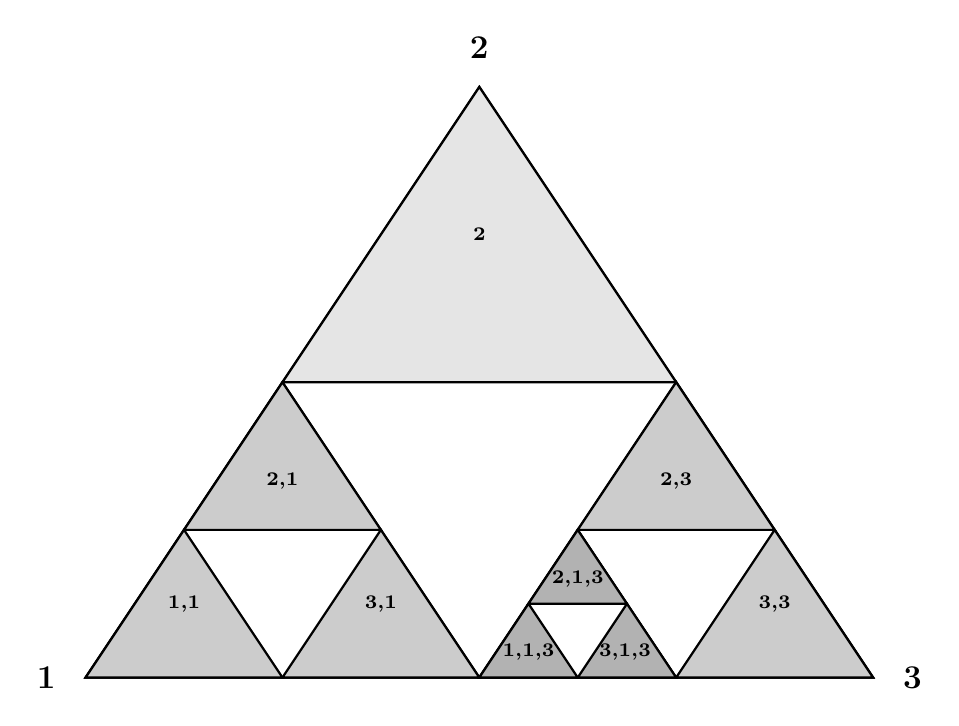
\begin{tikzpicture}
    \draw[thick] (0,0) -- (10,0) -- (5,7.5) -- cycle;
    
    \draw[thick] (0,0) -- (5,0) -- (2.5,3.75) -- cycle;  
    \draw[thick] (10,0) -- (5,0) -- (7.5,3.75) -- cycle;
    \draw[thick, fill=black!10] (2.5,3.75) -- (7.5,3.75) -- (5,7.5) -- cycle;

    
    \draw[thick, fill=black!20] (0,0) -- (2.5,0) -- (1.25,1.875) -- cycle;
    \draw[thick, fill=black!20] (2.5,0) -- (5,0) -- (3.75,1.875) -- cycle;
    \draw[thick, fill=black!20] (1.25,1.875) -- (3.75,1.875) -- (2.5,3.75) -- cycle;
    \draw[thick] (5,0) -- (7.5,0) -- (6.25,1.875) -- cycle;
    \draw[thick, fill=black!20] (7.5,0) -- (10,0) -- (8.75,1.875) -- cycle;
    \draw[thick, fill=black!20] (6.25,1.875) -- (8.75,1.875) -- (7.5,3.75) -- cycle;
    
    
    \draw[thick, fill=black!30] (5,0) -- (6.25,0) -- (5.625,0.9375) -- cycle;
    \draw[thick, fill=black!30] (6.25,0) -- (7.5,0) -- (6.875,0.9375) -- cycle;
    \draw[thick, fill=black!30] (5.625,0.9375) -- (6.875,0.9375) -- (6.25,1.875) -- cycle;

    \node at (5,5.625) {\scriptsize\textbf{2}};
    \node at (5,8) {\large\textbf{2}};
    \node at (-0.5,0) {\large\textbf{1}};
    \node at (10.5,0) {\large\textbf{3}};
    
    \node at (1.25,0.9375) {\scriptsize\textbf{1,1}};
    \node at (2.5, 2.5) {\scriptsize\textbf{2,1}};
    \node at (3.75, 0.9325) {\scriptsize\textbf{3,1}};
    
    \node at (7.5, 2.5) {\scriptsize\textbf{2,3}};
    \node at (8.75, 0.9325) {\scriptsize\textbf{3,3}};
    
    \node at (5.625, 0.32625) {\scriptsize\textbf{1,1,3}};
    \node at (6.25, 1.25) {\scriptsize\textbf{2,1,3}};
    \node at (6.85, 0.32625) {\scriptsize\textbf{3,1,3}};

\end{tikzpicture}
\end{center}
\caption{A pictorial representation of a chaos game to generate a Sierpinski Triangle. A point is chose at random from the outermost triangle then, at each iteration, is updated halfway towards a randomly selected vertex. The triangle marked $3,1,3$ represents the area the randomly selected first point must be if the sequence of vertices has been first $3$, then $1$ then $3$. Repeated ad infinitum will generate a Sierpinski Triangle.}  \label{fig:chaos_game}
\end{figure}

Finally, the Optimised Model appears to be failing to live up to its name. While it does induce a reduction in the entropy of the system, it does not enable the agents to become certain that any one state is true. That said, the agents do arrive at a consensus, as evidenced by the J Divergence plot. This indicated that the agents converge to a single spot in probability space, but that that spot is not certainty in a single state. Let us take an example run of the Optimised Model, in \cref{fig:optimised_problem_case}. 

\begin{figure}[H]
    \centering
    \includegraphics[width=0.49\textwidth]{Images/Figures/Barycenter/Optimised_problem_case.png}
    \caption{ A Barycenter plot showing $100$ agents in a world with 3 states at time $t=10,000$. \textit{Computed using $\alpha = 0.3, n=3$} }
    \label{fig:optimised_problem_case}
\end{figure}

Here, the agents appear to have converged to and remained at the uncertain result

\begin{center}
$\mathbf{P}^t \approx \begin{bmatrix}
    \alpha & 1 - \alpha & 0 \\
    \alpha & 1 - \alpha & 0 \\
    \vdots & \vdots & \vdots \\
    \alpha & 1 - \alpha & 0
\end{bmatrix}$
\end{center}

In order to better understand this phenomenon, we must return to the objective function of this mode. Since the speaker seeks to minimise the J Divergence between themselves and the listener, at this final state, if the speaker were to assert a single state, the listener would likely become more certain in that single state, gradually allowing the population to become certain of the true state of the world. However, if the speaker were to assert the singleton, the J Divergence between the speaker and listener would clearly increase, so it serves the speaker to assert something that does not cause the speaker to move away, even if this were to improve the collective certainty. 



\subsubsection{Convergence}

In order to compare the behaviour of the non-trivial models, let us examine their convergent behaviour across a range of parameter values. First, we consider varying $\gamma$ between zero and one for the Bottom Up and Top Down models as $\gamma$ does not affect the other speaker models. Recall that the system is said to have converged if $\Delta \hat{E}^{T+t} = \abs{ \hat{E}^t -  \hat{E}^{t+T}}  \leq \eta$. \Cref{fig:convergence_none} shows some examples. 

\begin{figure}[H]
 \centering
  \begin{subfigure}[ht]{0.45\textwidth}
    \includegraphics[width=\textwidth]{Images/Figures/All/Convergence_ALL_n_3_p_100_gamma_100_runs_20.png}
    \caption{Convergence}\label{fig:convergence}
 \end{subfigure}
 \hfill
 \begin{subfigure}[ht]{0.45\textwidth}
    \includegraphics[width=\textwidth]{Images/Figures/All/J_Div_ALL_n_3_p_100_gamma_100_runs_20.png}
    \caption{J-Divergence}\label{fig:J-Div_convergence}
 \end{subfigure}
 \hfill
 \begin{subfigure}[ht]{0.45\textwidth}
    \includegraphics[width=\textwidth]{Images/Figures/All/Entropy_ALL_n_3_p_100_gamma_100_runs_20.png}
    \caption{Entropy}\label{fig:entropy_convergence}
 \end{subfigure}
 \caption{Three plots showing time to (a) convergence, (b) entropy and (c) J-Divergence at steady state against a range of values for $\gamma$ for the Bottom Up and Top Down model. }\label{fig:convergence_none}
\end{figure}

It is apparent that, for both models, high values of $\gamma$ relate to very rapid convergence. This can be attributed to the fact that at values of $\gamma \approx 1$, it is impossible for either model to create a meaningful assertion; they are limited to asserting $\emptyset$ in the Bottom Up model and $\mathbf{W}$ for the Top Down which are both produce no reaction from the listening agent. This registers as very rapid convergence since the entropy does not change over time. 
In the the Bottom Up plots, one can observe that we get rapid convergence for values of $\gamma \geq \frac{1}{2}$. At this point, it becomes impossible for the speaker to assert anything other than a singleton, meaning that its arguments are guaranteed to be precise. This alone will increase the rate of convergence, but another factor to consider is that as gamma increases, the only agents that can put forward any non-trivial argument are those who already hold extreme beliefs which high probability in one particular state. This accelerates the movement of the general population towards the region in which extremist speakers can speak until more and more of the population holds similarly strong beliefs and so more of them become able to assert something, perpetuating the effect. 

In the Bottom Up plots it is also possible to observe a sharp increase in convergence time shortly after $ \gamma = \frac{1}{n}$. As $\gamma$ increases above this point, it begins to create a region of probability space in which it is impossible for an agent to assert anything, making them purely passive, voiceless. For instance, if $\mathbf{P}_S =\{ 0.3, 0.3, 0.4\}$ and $\gamma = 0.5$, it is impossible for the speaker to assert anything. This will increase the convergence time as, if such an agent is picked, it is incapable of speaking, meanwhile, the agents that can speak are likely to be asserting slightly general statements so convergence is slow until $\gamma$ approaches $\frac{1}{2}$. 

The top down approach exhibits some different behaviour with slow convergence times for low values of gamma that appear to decrease for the most part. The slow convergence for low $\gamma$ is attributable oscillations in the dynamics of the system. At these low values, it becomes possible for the agents to assert states for which they have very little probability. This delays convergence by convincing listening agents to update their probability distributions in a way that increases the distance between the speaker and listener. 

The entropy and divergence plots reveal the state of the agents at time of convergence. High entropy implies that some agents do not have strong belief in one state, whereas the average pairwise J-Divergence suggests that they have failed to converge on a single state of the world. It can be seen that, for low values of gamma, we get a variety of different beliefs in the population, and that at least some of them are not certain in one state of the world alone. This is due to the lack of ability in the speaker to create non-zero arguments in the Bottom Up model, but as gamma increases there is a clear decrease in both entropy and J-divergence as both models find more flexibility in their expressions. As $\gamma$ increases, the Bottom Up model becomes less able to express its beliefs, and the extreme speakers are the only ones able to speak, decreasing the convergence times but, as the probability of the entropy changing very little over a number of iterations increases, so does the entropy and J-divergence. 

The Top Down model is shown to be more robust to changes in $\gamma$, with the majority of the agents holding strong beliefs at convergence, although they do not always agree on the strong belief as evidenced by the relatively high value of J-divergence. 


\subsection{Analysis of Listener Models}

The previous analyses have dealt with the solely Simple listeners. Here we explore the effects of introducing the other types of listener we defined above. In order to maintain parity between the speaker and listener behaviour, the Discerning and Spiteful models disagree with an assertion if it fails to satisfy the reversal of the process that created it. In order to analyse these models, the above figures have been replicated, with different listener models. \Cref{fig:convergence_FIE} shows the convergence of discerning listeners. 

\todo[inline]{Replot these figures without Open and Optimised as they are unaffected by $\gamma$}

\begin{figure}[H]
 \centering
  \begin{subfigure}[ht]{0.45\textwidth}
    \includegraphics[width=\textwidth]{Images/Figures/ListenerModelPlots/FIE/Convergence.png}
    \caption{Convergence}
 \end{subfigure}
 \hfill
 \begin{subfigure}[ht]{0.45\textwidth}
    \includegraphics[width=\textwidth]{Images/Figures/ListenerModelPlots/FIE/J-Div.png}
    \caption{J-Divergence}
 \end{subfigure}
 \hfill
 \begin{subfigure}[ht]{0.45\textwidth}
    \includegraphics[width=\textwidth]{Images/Figures/ListenerModelPlots/FIE/Entropy.png}
    \caption{Entropy}
 \end{subfigure}

 \caption{Three plots showing time to convergence, entropy and J-Divergence at convergence against a range of values for $\gamma$ for the Open, Bottom Up, Top Down and Optimised models, with discerning listeners.} \label{fig:convergence_FIE}
\end{figure}


From this figure it can be clearly seen that both the Open and Optimised models do not depend on $\gamma$ and so are approximately constant in these plots. As above, they both demonstrate agents converging to very similar beliefs although neither manages to achieve certainty. 

\todo[inline]{maybe break paragraph up}
Here, the Bottom Up and Top Down models behave differently, converging as quickly as the Open model for low values of $\gamma$. However, for the same values of $\gamma$ the J-Divergence appears to be maximal, suggesting that there is not a consensus in the population, although the entropy indicates certainty. This corresponds with the agents dividing into camps that are certain in one state of the world that are incapable of listening to the assertions of those they are at odds with.  As $\gamma$ increases above $0.5$, the J-Divergence begins to decrease as more and more agents become able to listen to a wider set of assertions, while simultaneously increasing the entropy in the system as those assertions become more general, including more states and so becoming less informative. As $\gamma \approx 0.6$, it can be seen that the Bottom Up model begins to converge much more rapidly, while the J-Divergence and entropy plots begin to plateau. Since $\gamma$ represents the threshold above which the speaker can assert a state, it is intuitive that as the threshold rises, the speaker is more and more limited in what they can assert. It is in this region that the Bottom Up beings to be unable to assert anything other than $\emptyset$ and so the agents converge more rapidly, though their opinions are still scattered and diverse. This does not appear to be the case for the Top Down model as the convergence times undergo a slight increase in this region, corresponding with a momentary plateau in J-Divergence and entropy. This is likely due to the fact that for high values of $\gamma$, the listener is more likely to disregard assertions, including agents with relatively uncertain beliefs as they are unable to update on any argument. Since the assertion of every state does not persuade the listener of anything, only assertions with $\abs{\mathbf{A}} < n$ are informative, however, uncertain agents in a world with $\gamma > \frac{n-1}{n}$ are unlikely to find any arguments they can update on, hence the deviation at $\gamma \approx 0.6$. Meanwhile, agents that are already confident in one state are still able to update, though, as $\gamma$ increases further, they become fewer and fewer. 

These results show that, when the listeners are capable of disregarding the assertions of a speaker, the population becomes divided, though converged. Furthermore, the Top Down model is slightly more robust a solution for a wider range of $\gamma$. This is likely due to its greater level of flexibility built into the model. 

We now consider the convergence when the population comprised of Spiteful listeners

\todo[inline]{Also redo these figures, especially as the legend is obscuring some convergence}


\begin{figure}[H]
 \centering
  \begin{subfigure}[ht]{0.45\textwidth}
    \includegraphics[width=\textwidth]{Images/Figures/ListenerModelPlots/Spiteful/Convergence.png}
    \caption{Convergence}
 \end{subfigure}
 \hfill
 \begin{subfigure}[ht]{0.45\textwidth}
    \includegraphics[width=\textwidth]{Images/Figures/ListenerModelPlots/Spiteful/J-Div.png}
    \caption{J-Divergence}
 \end{subfigure}
 \hfill
 \begin{subfigure}[ht]{0.45\textwidth}
    \includegraphics[width=\textwidth]{Images/Figures/ListenerModelPlots/Spiteful/Entropy.png}
    \caption{Entropy}
 \end{subfigure}
 \caption{Three plots showing time to convergence, entropy and J-Divergence at convergence against a range of values for $\gamma$ for the Bottom Up and Top Down model, with discerning listeners. (\textit{$\alpha = 0.5, N = 100$ averaged over 20 runs. Convergence is defined as above using $t=100, \epsilon = 1\times10^{-5}$})}\label{fig:convergence_Spite}
\end{figure}

These plots again show the division formed by having listeners that can disregard speakers assertions. The J-Divergence plot shows that for all but the extreme values of $\gamma$, the agents disagree, forming highly separated beliefs. The entropy plot shows that these separate beliefs are again certain ones, suggesting that the agents reside in different corners of the simplex. The first main difference between the Discerning and Spiteful plots is here the Bottom Up model fails to converge for some low values of $\gamma$. This is due to the fact that, for these values, both the constraints on what the speakers may assert and what the listener may update on are loose, allowing for a high degree of changeability between iterations. The Bottom Up model also suffers at high values of $\gamma$ as, again, the speakers become less able to assert anything at all. 




Finally, let us consider an increasingly stubborn population. Here, the population places less and less importance on new information as they receive each new argument. This promotes the ossification of beliefs. \Cref{fig:convergence_Ageing} shows the convergence plots. 


\begin{figure}[H]
 \centering
  \begin{subfigure}[ht]{0.45\textwidth}
    \includegraphics[width=\textwidth]{Images/Figures/ListenerModelPlots/Ageing/Convergence.png}
    \caption{Convergence}
 \end{subfigure}
 \hfill
 \begin{subfigure}[ht]{0.45\textwidth}
    \includegraphics[width=\textwidth]{Images/Figures/ListenerModelPlots/Ageing/J-Div.png}
    \caption{J-Divergence}
 \end{subfigure}
 \hfill
 \begin{subfigure}[ht]{0.45\textwidth}
    \includegraphics[width=\textwidth]{Images/Figures/ListenerModelPlots/Ageing/Entropy.png}
    \caption{Entropy}
 \end{subfigure}
 \caption{Three plots showing time to convergence, entropy and J-Divergence at convergence against a range of values for $\gamma$ for the Open, Bottom Up, Top Down and Optimised models, with stubborn listeners. (\textit{$\alpha_0 = 0.5, N = 100, \lambda = 0.002$ averaged over 20 runs. Convergence is defined as above using $T=100, \eta = 1\times10^{-5}$})}\label{fig:convergence_Ageing}
\end{figure}

These graphs show that the Top Down model approximates the Optimised model, demonstrating very little dependence on $\gamma$. It regularly converges after $8,000$ iterations or so, seemingly an upper limit 

\todo[inline]{These plots need to be run again, $\lambda$ was too small so the effect of time was minimal}



The results presented above demonstrate that when agents openly express the exact nature of their beliefs, the population becomes uncertain. However, when they express arguments as certain states of the world, it becomes possible for the population as a whole to converge on a single state, provided the listener agents are indiscriminate in the information they use to update their beliefs. The Bottom Up and Top Down approaches achieve similar results, however, the Bottom Up approach is rendered ineffective for large values for $\gamma$. The Top Down model allows speakers to be more flexible with their assertions, allowing the majority of agents to reach certainty in a state at convergence. It is unclear whether either of these models outperforms the other, however it can be shown that the inclusion of discerning agents has a remarkable effect. When listeners ignore assertions that they do not already believe to have a degree of truth in it, they disregard it. This results in agents converging to distinct and certain probability distributions, sitting in opposing corners of a Barycenter plot, refusing to listen to any argument from another vertex.  